% -------------------------------------------------------------------------------
% Establish page structure & font.
\documentclass[12pt]{report}

\usepackage[total={6.5in, 9in},
	left=1in,
	right=1in,
	top=1in,
	bottom=1in,]{geometry} % Page structure

\usepackage{graphicx} % Required for inserting images
\graphicspath{{../../.images/}} % Any additional images I use (BCU logo, etc) are from here.

\usepackage[utf8]{inputenc} % UTF-8 encoding
\usepackage[T1]{fontenc} % T1 font
\usepackage{float}  % Allows for floats to be positioned using [H], which correctly
                    % positions them relative to their location within my LaTeX code.
\usepackage{subcaption}

% -------------------------------------------------------------------------------
% Declare biblatex with custom Harvard BCU styling for referencing.
\usepackage[
    useprefix=true,
    maxcitenames=3,
    maxbibnames=99,
    style=authoryear,
    dashed=false, 
    natbib=true,
    url=false,
    backend=biber
]{biblatex}

% Additional styling options to ensure Harvard referencing format.
\renewbibmacro*{volume+number+eid}{
    \printfield{volume}
    \setunit*{\addnbspace}
    \printfield{number}
    \setunit{\addcomma\space}
    \printfield{eid}}
\DeclareFieldFormat[article]{number}{\mkbibparens{#1}}

% Declare it as the bibliography source, to be called later via \printbibliography
\addbibresource{pipeline.bib}

% -------------------------------------------------------------------------------
% To prevent "Chapter N" display for each chapter
\usepackage[compact]{titlesec}
\usepackage{wasysym}
\usepackage{import}

\titlespacing*{\chapter}{0pt}{-2cm}{0.5cm}
\titleformat{\chapter}[display]
{\normalfont\bfseries}{}{0pt}{\Huge}

% -------------------------------------------------------------------------------
% Custom macro to make an un-numbered footnote.

\newcommand\blfootnote[1]{
    \begingroup
    \renewcommand\thefootnote{}\footnote{#1}
    \addtocounter{footnote}{-1}
    \endgroup
}

% -------------------------------------------------------------------------------
% Fancy headers; used to show my name, BCU logo and current chapter for the page.
\usepackage{fancyhdr}
\usepackage{calc}
\pagestyle{fancy}

\setlength\headheight{37pt} % Set custom header height to fit the image.

\renewcommand{\chaptermark}[1]{%
    \markboth{#1}{}} % Include chapter name.


% Lewis Higgins - ID 22133848           [BCU LOGO]                [CHAPTER NAME]
\lhead{Lewis Higgins - ID 22133848~~~~~~~~~~~~~~~
\includegraphics[width=1.75cm]{BCU}}
\fancyhead[R]{\leftmark}

% ------------------------------------------------------------------------------
% Used to add PDF hyperlinks for figures and the contents page.

\usepackage{hyperref}

\hypersetup{
    colorlinks=true,
    linkcolor=black,
    filecolor=magenta,
    urlcolor=blue,
    citecolor=black,
}

% ------------------------------------------------------------------------------
\usepackage{xcolor} 
\usepackage{colortbl}
\usepackage{longtable}
\usepackage{amssymb}
% ------------------------------------------------------------------------------


% -------------------------------------------------------------------------------

\title{CMP6230 Draft Pipeline}
\author{Lewis Higgins - Student ID 22133848}
\date{November 2024}

% -------------------------------------------------------------------------------

\begin{document}


\makeatletter
\begin{titlepage}
    \begin{center}
        
\includegraphics[width=0.7\linewidth]{BCU}\\[4ex]
        {\huge \bfseries  \@title }\\[50ex]
        {\@author}\\[30ex]
    \end{center}
\end{titlepage}
\makeatother
\thispagestyle{empty}
\newpage


% Page counter trick so that the contents page doesn't increment it.
\setcounter{page}{0}

\tableofcontents
\thispagestyle{empty}


\chapter{Candidate Data Sources}
For the first stage of the pipeline, data ingestion, three data sources will be identified in order to find 
the one that would be most optimal for the production and deployment of a machine learning model to complete 
a supervised learning task.

% \section{Notes - DELETE BEFORE SUBMISSION}
% Lucidchart can generate ERDs from CSVs.
% For each, show the pandas head, column data types and ERD.
% Finding one with multiple CSVs can be good to make the ERD look more complex. 
% \textbf{So far, all of your data is from Kaggle. Consider another source like data.gov.uk, especially
% considering that it can give you raw data for preprocessing.} On Kaggle, the "Provenance" section will 
% have the source if the description doesn't. If neither have a source, it's probably fake data.

% \begin{itemize}
%     \item Smoke detection \begin{itemize}
%         \item Real data
%         \item Lots to explain (how the alarms work etc)
%         \item Preprocessed, but you could still do more (remove timestamp etc)
%         \item Classification - Should the smoke/fire alarm sound?
%     \end{itemize}
%     \item Employee data \begin{itemize}
%         \item Allegedly real data though it seems hard to believe.
%         \item Classification - Is the employee likely to find another job instead?
%     \end{itemize}
%     \item Australian weather \begin{itemize}
%         \item Promising. Real data, but very large. Can do lots of preprocessing.
%         \item Classification - Will it rain tomorrow?
%     \end{itemize}
%     \item Cardiovascular disease \begin{itemize}
%         \item Good data, enormous amount of it (laptop might not handle it), good source. 
%         \item However, it's already been processed. Check if that's fine or not.
%         \item Classification - Do they have heart disease?
%     \end{itemize}
%     \item Diabetes \begin{itemize}
%         \item In consideration for CMP6200, cannot use a dataset in both.
%         \item It's actually real data according to the Kaggle page, from "multiple healthcare providers" and the 
%         electronic health records (EHRs) they keep.
%         \item Preprocessed already, but duplicates exist in it.
%         \item Only 9 features, is that a bad thing?
%         \item Classification - Do they have diabetes?
%     \end{itemize}
%     \item Indian Liver Patients \begin{itemize}
%         \item Alternative source [OpenML]
%         \item Alternative file format [ARFF]
%         \item 900 rows
%         \item Classification - Are they a liver patient?
%         \item Good option mostly due to alt file format. Unfortunately still OBT though.
%     \end{itemize}
%     \item Student performance \begin{itemize}
%         \item Data from two unnamed Portugeuse schools
%         \item Lots of columns, perhaps too many.
%     \end{itemize}
% \end{itemize}

% All tasks of sheet 1, sheet 2 "should be analysed and you should write the plan for it", because sheet 2
% refers moreso to the final report itself due both Dec 13 (draft) and Jan 10 (final).
% Because the amount of rows is not relevant in this particular module, you can use smaller ones 
% like the 305 row Heart set.
% Week 8's lab is likely to be of vital importance to the final assessment of this module, as it 
% goes through the use of MLFlow. 

% \textbf{It's infeasible to do this on your laptop. Tuesday and Wednesday you'll need to smash this out
% \textit{quickly.}}

% #############################################################################
% GENERAL TODO: 
%
% All Entity Relationship Diagrams. 
% General polish.
% Use more terminology (nominal data, etc)
% Add some more href links, especially for candidate 1.
% Maybe don't have datasets as citations but rather as links.
% Attempt to find a dataset that's not a flat-file CSV.
% If you do the ERDs, the tables probably don't need the data types.
% #############################################################################

\section{Candidate 1 - Indian Liver Patient Dataset}
\href{https://archive.ics.uci.edu/dataset/225}{This dataset} \autocite{bendi_ramana_ilpd_2022} consists of real data sourced from hospitals northeast of Andhra Pradesh in India. It was obtained from the
UCI Machine Learning Repository, and has been previously used by \textcite{straw_investigating_2022} in their analysis of sex-related bias in supervised learning models. The UCI ML Repository is a popular host of datasets used by students, 
educators and researchers worldwide for machine learning \autocite{uci_machine_learning_repository_about_nodate}, and hosts these datasets 
on the cloud for public download and usage, as long as credit is given. This dataset in particular aims to assist in the diagnosis of liver
disease due to increasing mortality rates from conditions like liver cirrhosis, and contains 584 records with 10 features
as well as the "Selector" classification column, where those wihout liver disease are classed as 1, and those with liver disease 
are classed as 2. For the purposes of the ML model, these can be changed to 0 and 1 respectively. 
The dataset is a single flat-file Comma-Seperated Values (CSV) file, which stores data by seperating each column with commas
and each row with line breaks. This CSV file uses a One Big Table (OBT) schema, as seen in the entity relationship diagram 
in Figure \ref{fig:ILPD-ERD}, wherein all of the data within this dataset is stored in a single table. % Do the ERD at some point.
Descriptions of the columns in the dataset, as well as the associated data types, can be found in Table \ref{tab:ILPD-Types}.

\begin{figure}[H]
    \centering
    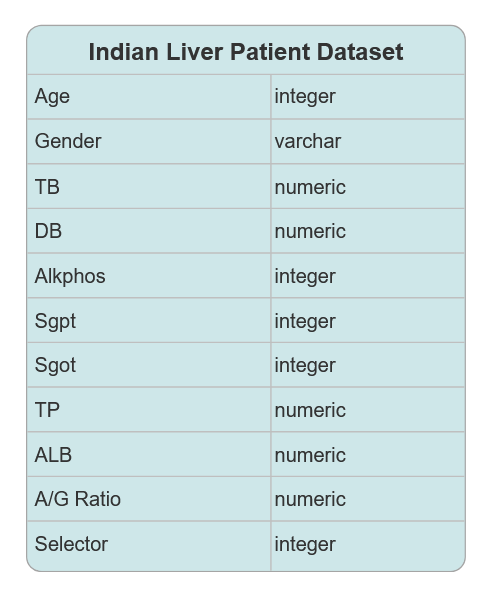
\includegraphics[width=.75\linewidth]{ILPD-ERD.png}
    \caption{An entity relationship diagram of the Indian Liver Patient Dataset.}
    \label{fig:ILPD-ERD}
\end{figure}


A minor issue with this file is that it has no headers in its CSV file, meaning that when imported, Pandas will interpret the first 
row of data as the names of the columns, though this can be combated by adding the "names" argument when calling Pandas' "read\_csv" function,
seen below in Figure \ref{fig:pandasNames}. 

\begin{figure}[H]
    \centering
    \begin{subfigure}{0.75\textwidth}
       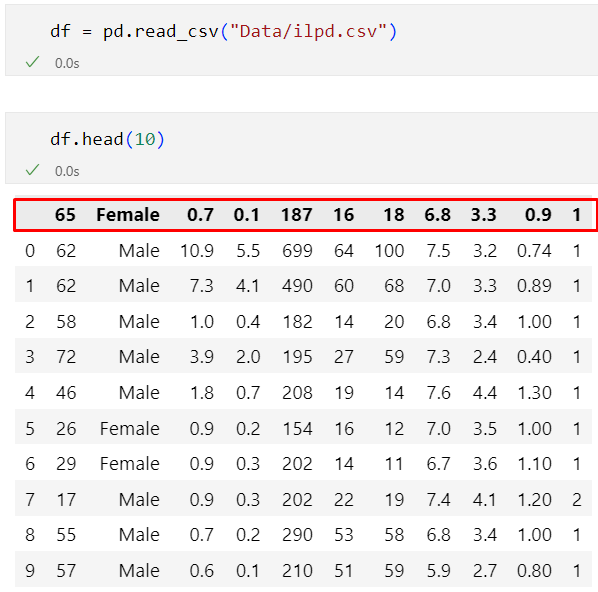
\includegraphics[width=1\linewidth]{pandasNoNames.png}
       \caption{Importing without supplying column names.}
       \label{fig:pandasNames} 
    \end{subfigure}
    
    \begin{subfigure}{1\textwidth}
       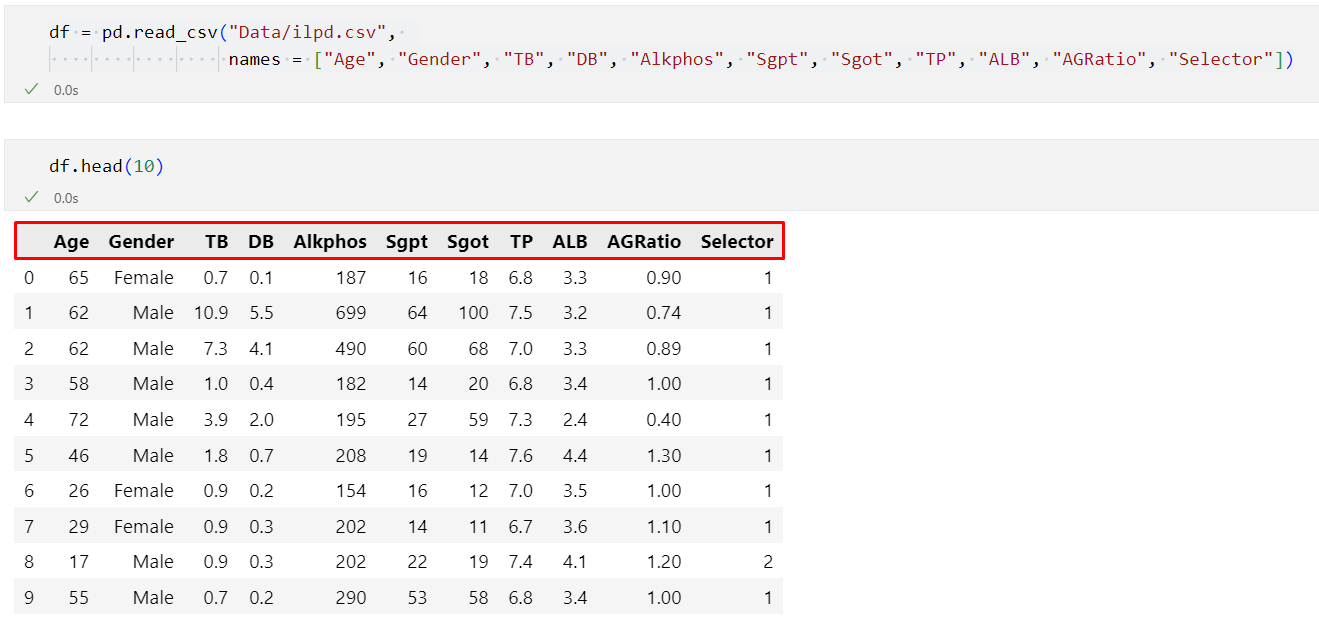
\includegraphics[width=1\linewidth]{pandasNames.png}
       \caption{Importing with the column names.}
       \label{fig:PN2}
    \end{subfigure}
    \caption{Importing the erroneous CSV using Pandas. The column headers are highlighted in a red box.}
\end{figure}

\begin{table}[H]
    \centering
        \begin{tabular}{ |p{0.4\textwidth}| p{0.45\textwidth}|}
            \hline
            \cellcolor{blue!25}Column & \cellcolor{blue!25}Description\\
            \hline
            Age & The patient's age. \textbf{Ages of 90 or over were listed as 90 before this dataset was published.} \\
            \hline
            Gender (Binary) & The patient's gender, either "Male" or "Female".\\
            \hline
            TB & Total bilirubin. Bilirubin is a substance produced by the liver, and a high presence of it may be indicative of
            liver problems \autocite{mayo_clinic_bilirubin_nodate}.\\
            \hline
            DB & Direct bilirubin. This is a slightly different form of bilirubin that is formed after the liver has processed it.\\
            \hline
            Alkphos & Levels of alkaline phosphate - an enzyme in the body produced by the liver. Too much may indicate liver disease. \autocite{clevelandclinic_alkaline_nodate}\\
            \hline
            Sgpt & Another enzyme found in the liver, where too much can indicate liver problems.\\
            \hline
            Sgot & Levels of AST in the blood, where too much indicates liver problems.\\
            \hline
            TP & Total proteins.\\
            \hline
            ALB & Albumin - a protein in blood plasma. Too little of this may indicate liver problems.\\
            \hline
            A/G Ratio & The ratio of albumin to globulin, which is another blood protein.\\
            \hline
            Selector & The classifier, indicating if the person has liver disease. The target column for the ML model.\\
            \hline
    \end{tabular}
    \caption{The data types of each column in the Indian Liver Patient Dataset.}\label{tab:ILPD-Types}
\end{table}

This dataset can be used to develop a supervised machine learning model for binary classification using the ten predictor 
variables and the ground truth Selector column, which will be used in measuring the accuracy of the model. There is a clear 
positive purpose for developing such a model; as previously mentioned, mortality rates from liver disease are high, and an early
diagnosis that could leverage the power of machine learning can greatly enhance the odds of successful treatment.


% \section{Candidate 2 - Cardiovascular Disease Dataset}
% The second dataset is also a real dataset of heart disease patients from four areas worldwide: Ohio, Hungary, Switzerland, and Virginia,
% and was identified through the UCI ML repository. The dataset consists of 14 features and a classifier column, with the data types and descriptions of each 
% shown in Table \ref{tab:Heart-Types}. The overall purpose of this dataset is for the analysis and diagnosis of heart disease, which is the leading 
% cause of death for both men and women in the US \autocite{cdc_heart_2024}. Unlike Candidate 1, this dataset consists of four seperate CSV files, where each CSV is for one of the 
% aforementioned locations. 

% \begin{table}[H]
%     \centering
%         \begin{tabular}{ |p{0.2\textwidth}|p{0.2\textwidth}| p{0.35\textwidth}|}
%             \hline
%             \cellcolor{blue!25}Column & \cellcolor{blue!25}Format & \cellcolor{blue!25}Description\\
%             \hline
%             Patient Identification Number & Integer & The patient's unique ID. This won't be used as a predictor because it has no affiliation. \\
%             \hline
%             Age & Integer & The patient's age.\\
%             \hline
%             Gender & Integer (Binary) & The patient's gender, where 0 is female and 1 is male. \\
%             \hline
%             Chest pain type & Integer (Nominal) & The type of pain the patient has, where 0 is typical angina, 1 is atypical angina, 2 is pain that is not angina, and 3 is no pain.\\
%             \hline
%             Resting blood pressure & Integer & The patient's blood pressure (It is not stated if this is their systolic or diastolic pressure).\\
%             \hline
%             Serum cholesterol & Integer & Total cholesterol in the blood. Too much can clog arteries and cause heart disease and/or attacks.\\
%             \hline
%             Fasting blood sugar & Integer (Binary) & 0 if under 120mg/dl, 1 if over 120mg/dl.\\
%             \hline
%             Resting ECG results & Integer (Nominal) & 0 if normal, 1 if ST-T wave abormality (irregular beat), 2 if ventricular hypertrophy.\\
%             \hline
%             Maximum heart rate & Integer & The highest heart rate documented for the patient.\\
%             \hline
%             Exercise induced angina & Integer (Binary) & 0 if they do not get chest pain during exercise, 1 if they do.\\
%             \hline
%             Oldpeak & Float & The difference in ST depression (a particular part of the heart's beating motion) when exercising compared to resting.\\
%             \hline
%             ST segment slope & Integer (Nominal) & The trend in the patient's ST segment reading, where 1 is upsloping, 2 is flat and 3 is downsloping. \\
%             \hline
%             Classifier & Integer (Binary) & If the patient has heart disease or not (0 if no, 1 if yes).\\
%             \hline
%     \end{tabular}
%     \caption{The data types of each column in the Cardiovascular Disease Dataset.}\label{tab:Heart-Types}
% \end{table}

\section{Candidate 2 - Loan Approval Classification Dataset}
\href{https://www.kaggle.com/datasets/taweilo/loan-approval-classification-data}{This dataset} was sourced from Kaggle's cloud servers under 
an Apache 2.0 license, which states that the dataset can be used as long as credit is given to the original author,
and takes the form of a flat-file CSV using a One Big Table schema. Unlike Candidate 1, this dataset does not consist of real data, and 
instead consists of synthetic data. This is likely due to the fact that this dataset, if it used real data, would contain extremely personal 
information that could not be shared online due to legislation such as GDPR. This particular dataset is an enhanced version of \href{https://www.kaggle.com/datasets/laotse/credit-risk-dataset}{a different credit risk dataset},
which also did not provide an original source and is presumably synthetic data. The dataset consists of 45,000 records and 14 features, with 
one of these being the ground truth target variable "loan\_status", which is whether the person should be given a loan or not. As such, it is well suited 
for a binary classification model, using the first 13 features as predictor variables. This can also be observed from the 28 notebooks on Kaggle that 
utilise this dataset. The data types for each column can be seen in the entity relationship diagram in Figure \ref{fig:Loan-ERD} and 
descriptions of each column can be seen in Table \ref{tab:Loan-Types}.

\begin{figure}[H]
    \centering
    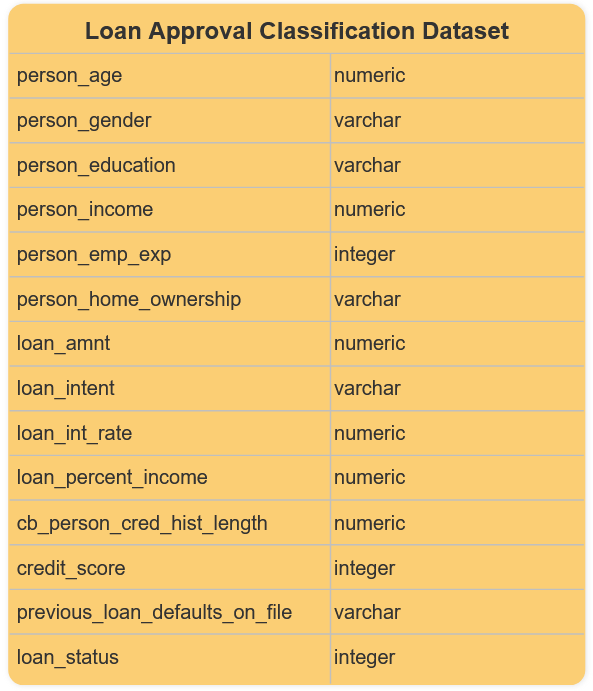
\includegraphics[width=.75\linewidth]{Loan-ERD.png}
    \caption{An entity relationship diagram of the Loan Approval Classification Dataset.}
    \label{fig:Loan-ERD}
\end{figure}


\begin{table}[H]
    \centering
        \begin{tabular}{ |p{0.4\textwidth}| p{0.425\textwidth}|}
            \hline
            \cellcolor{blue!25}Column & \cellcolor{blue!25}Description\\
            \hline
            person\_age & The age of the person.\\
            \hline
            person\_gender & The person's gender.\\
            \hline
            person\_education & The person's highest level of education.\\
            \hline
            person\_emp\_exp & The person's years of employment experience.\\
            \hline
            person\_home\_ownership & Home ownership status (for example rent, own, mortgage)\\
            \hline
            loan\_amnt & The amount of money requested.\\
            \hline
            loan\_intent & The purpose of the loan.\\
            \hline
            loan\_int\_rate & The interest rate of the loan.\\
            \hline
            loan\_percent\_income & Loan amount as a percentage of the person's yearly income.\\
            \hline
            cb\_person\_cred\_hist\_length & Length of credit history in years.\\
            \hline
            credit\_score & Credit score of the person.\\
            \hline
            previous\_loan\_defaults\_on\_file & If the person has defaulted on a loan before. \\
            \hline
            loan\_status & Whether the loan should be approved. 1 if yes, 0 if no.\\
            \hline
    \end{tabular}
    \caption{The descriptions of each column in the dataset.}\label{tab:Loan-Types}
\end{table}

\pagebreak

\section{Candidate 3 - Spotify Likes Dataset}
\href{https://www.kaggle.com/datasets/bricevergnou/spotify-recommendation/data}{This dataset} was sourced from \href{https://www.kaggle.com/datasets}{Kaggle}, a platform similar to the UCI ML repository in its purpose for students and researchers
that acts as a search engine for datasets, but also allows its users to host competitions, upload their machine learning models, and also upload 
their own Python notebooks. This dataset is stored on their servers on the cloud, and is free to download and use. The data itself is split over 
a CSV file and two JavaScript Object Notation (JSON) files, with all three utilising a One Big Table schema. JSON files 
store data in \textbf{key-value pairs}, such as in the example snippet of this dataset depicted in Figure \ref{fig:spotifySnippet}.  

\begin{figure}[H]
    \centering
    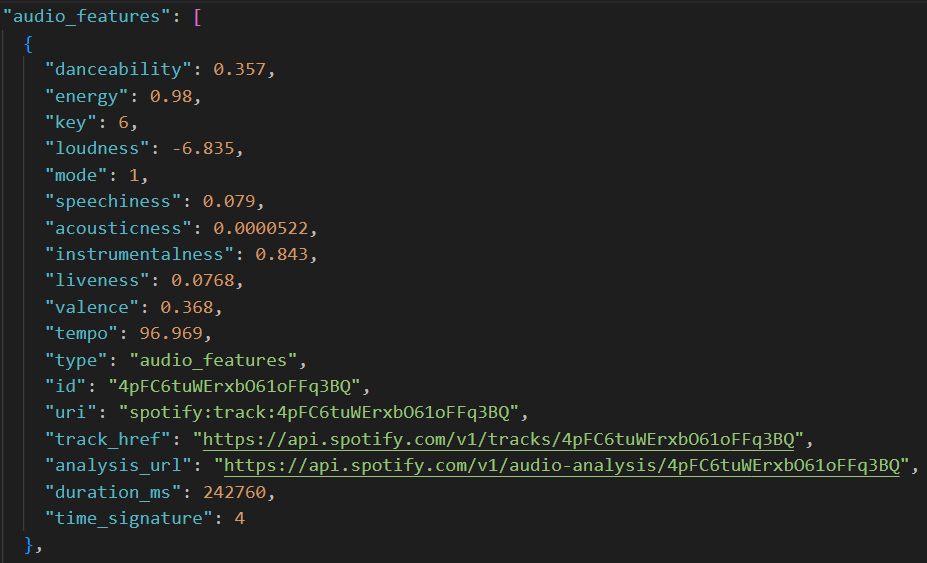
\includegraphics[width=.75\linewidth]{spotifySnippet.png}
    \caption{A snippet of the JSON data, viewed in Visual Studio Code.}
    \label{fig:spotifySnippet}
\end{figure}

Every row in the JSON files is part of the single "audio\_features" key, and each new row is seperated by curly braces \{\}. Each column is then given as a 
key-value pair, such as the first row in the image, where "danceability" is the key, and 0.352 is the associated value.

\noindent This dataset does consist of real data, sourced from the author's personal liked songs directly via the 
\href{https://developer.spotify.com/documentation/web-api}{Spotify API}. There are 195 rows of data, with 100 liked songs, and 95 disliked songs.
Liked and disliked songs are seperated into two JSON files, named "dislike" and "good". The two JSON files have 18 features, as depicted in Figure 
\ref{fig:JSON-ERD}. 

\begin{figure}[H]
    \centering
    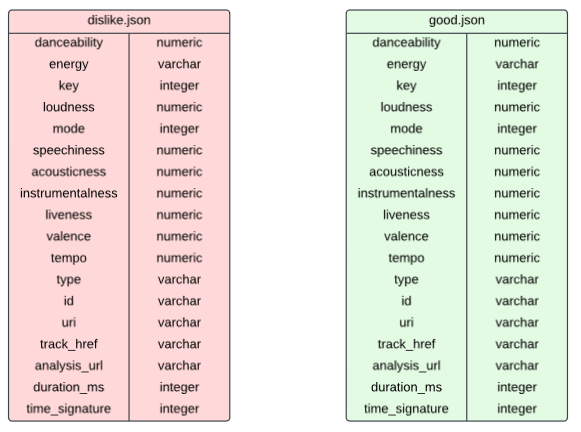
\includegraphics[width=.75\linewidth]{SpotifyJSON-ERD.png}
    \caption{An entity relationship diagram of the two JSON files. Data does not overlap between them, so they have no relation.}
    \label{fig:JSON-ERD}
\end{figure}

Before publicising this data, however, the author had done some preprocessing of their own, having included the additional CSV file,
produced as a result of merging the two JSON files into one CSV and removing unnecessary columns, as depicted in Figure \ref{fig:Spotify-ERD}.

\begin{figure}[H]
    \centering
    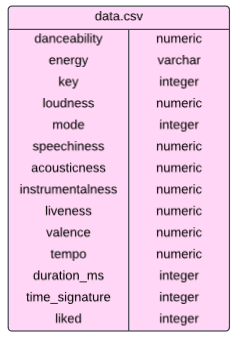
\includegraphics[width=.5\linewidth]{Spotify-ERD.png}
    \caption{An entity relationship diagram of the preprocessed CSV file.}
    \label{fig:Spotify-ERD}
\end{figure}

While a machine learning classification problem can definitely be performed on this dataset to identify if the author would like a song, 
it has significantly less of a positive impact than Candidates 1 and 2, as this dataset is the author's subjective belief rather than objective
fact that can be applied to other people. Nevertheless, the data types and descriptions of each column can be found in Table \ref{tab:Spotify-Types}.

\begin{table}[H]
    \centering
        \begin{tabular}{ |p{0.2\textwidth} | p{0.5\textwidth}|}
            \hline
            \cellcolor{blue!25}Column & \cellcolor{blue!25}Description\\
            \hline
            Danceability & How suitable a song is for dancing, calculated from the tempo, rhythm stability, beat strength and overall regularity. 1.0 means it is very danceable. \\
            \hline
            Energy & The intensity and activity of a song. For example, death metal is high energy, whereas classical music is low intensity. 1.0 is the most energetic.\\
            \hline
            Key & The musical key the song is in, converted to an integer using \href{https://smbutterfield.github.io/ibmt17-18/22-intro-to-non-diatonic-materials/b2-tx-pcintnotation.html}{standard pitch class notation.}\autocite{butterfield_22b_nodate} \\
            \hline
            Loudness & The averaged decibel volume of a song, typically between -60 and 0 dB.\\
            \hline
            Mode & Whether a song is in major or minor scale. 1 is major and 0 is minor.\\
            \hline
            Speechiness & The calculated presence of spoken words in a song.\\
            \hline
            Acousticness & A confidence measure from 0.0 to 1.0 of whether the track is acoustic. 1.0 represents high confidence the track is acoustic.\\
            \hline
            Instrumentalness & Whether a song has no vocals.\\
            \hline
            Liveness & Whether a live audience can be heard as part of a song.\\
            \hline
            Valence & The musical positiveness of a song.\\
            \hline
            Tempo & The beats per minute of a song.\\
            \hline
            Duration\_MS & The duration of a song in milliseconds.\\
            \hline
            Time signature & The estimated time signature of the song.\\
            \hline
            \cellcolor{red!15}Liked & The target variable, indicative of whether the author liked the song or not.\\
            \hline
            \cellcolor{green!15}Type & Always "audio\_features". Not a relevant predictor.\\
            \hline
            \cellcolor{green!15}ID & Spotify's own unique ID for a song. Not a relevant predictor.\\
            \hline
            \cellcolor{green!15}URI & Spotify's URI for the song. Not a relevant predictor.\\
            \hline
            \cellcolor{green!15}Track HREF & A link to the song on Spotify's API. Not a relevant predictor.\\  
            \hline
            \cellcolor{green!15}Analysis URL & A link to the song's audio analysis data. Not a relevant predictor. \\
            \hline
    \end{tabular}
    \caption{The descriptions of each column in the Spotify songs dataset \autocite{spotify_web_nodate}. Red columns are only present in the CSV, whereas green columns are only present in the JSONs.}\label{tab:Spotify-Types}
\end{table}

These measurements and the descriptions are \href{https://developer.spotify.com/documentation/web-api/reference/get-audio-features}{part of Spotify's API},
and are automatically calculated when songs are uploaded to the service. The ground truth of the dataset is present in the CSV file as the "liked" classifier 
column, and a train/test split can be implemented for predictions, which is aided by the fact that this dataset is well balanced (100 liked to 95 disliked).

\section{Chosen dataset}
AAAAA



\chapter{Planning the MLOps Pipeline}
All machine learning operations (MLOps) follow a five-step repeatable pipeline, outlined in Figure \ref{fig:MLPipeline}, where the output of one stage
becomes the input of the next. The pipeline begins with raw data and finishes with a trained machine learning model, and is often 
repeated at certain intervals, which could be as simple as once a day, or it could be repeated as new data becomes available. 
This repetition is performed automatically, so that the final model can become progressively more accurate. Because the process 
must be repeatable and automated, it is essential that data is validated to ensure that one run of the pipeline where the data may have 
been corrupted somehow would not cause issues, which would quickly spiral out of control as the pipeline is repeated again and again.
These validation procedures and the software utilised for them are documented in Section \ref{sec:Software}.
Overall, MLOps pipelines standardise the development and deployment process of machine learning models, ensuring continuous integration
(CI) and continuous delivery (CD) and enhancing collaboration between data scientists and development teams.

% --- Week 8 Thursday ---
% "The machine learning part is not important in this module, but rather the pipeline is."
% Don't answer the task sheet questions in a single sentence. You want to give a deep analysis of what it is,
% which I believe I've already done. Talk about why it was collected in the first place, which you have NOT done.

% References are expected in this report as seen in the examples. Emphasised that it's an ACADEMIC report.
% It's fine to use OBT datasets. Create an ERD. You could potentially create tables by splitting the OBT.

% Detailed discussion on the five stages. See sheet for questions you need to answer for each.
% Tools and techniques on a per-stage basis rather than their own section? Up to you.
% You can relate your explanations of the stages to your chosen dataset. "For example, in the selected dataset,
% this stage would be applied by..."

% An important part is WHO is involved. You've not really looked into that though it shouldn't be hard to find out.

% [I didn't even realise there was a third page of the sheet. Not ideal]
% Discussion of the selected dataset. Isn't it repeating the first section though?
% Will you store it in MariaDB or a "graph database" (?)
% Physical/logical structure of the data AFTER ingestion.
% She mentioned creating a star schema of the data. Could you? IF it's one with many features, maybe.

% This info is apparently all available within the first three weeks of the module.
% Remember that you missed Week 3, so if it was there you wouldn't know.

% Example shown in class is not listed on Moodle.
% They gave references to sources about what CSVs are and ERDs.
% You should probably do the same, and also give one for OBT as you never explained it.
% Just saying varchar without a character amount could be fine in the ERD.
% They made a table of comparisons between the three, with stuff like the data types.

% NO DESIGNATED WORD COUNT!
% You're writing a plan that will probably change in the next assessment?
% You do not need to do implementation here (though you can???)
% IF you do so, an extra ZIP is needed with the dataset and code.
% You should do that - add a ZIP with the datasets and a Jupyter notebook with brief analysis (heads, types, etc).

% Also, if Airflow stops working after installing MLFlow, FastAPI and Uvicorn, you need to uninstall and reinstall
% FLask. pip uninstall flask, pip install flask==2.2.5
% -------------------------


\begin{figure}[H]
    \centering
    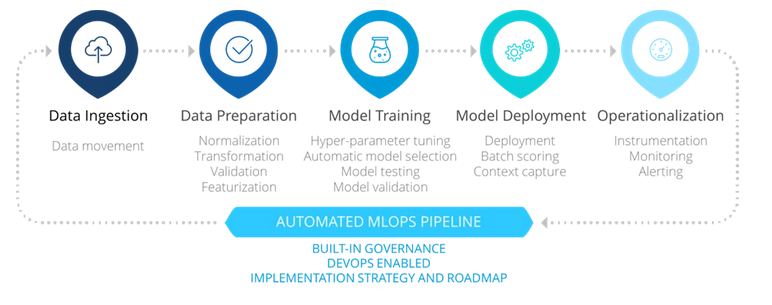
\includegraphics[width=.75\linewidth]{MLPipeline.png}
    \caption{The five key steps in an MLOps pipeline \autocite{incycle_software_mlops_nodate}.}
    \label{fig:MLPipeline}
\end{figure}

\section{Data Ingestion}
The first step of any machine learning pipeline is data ingestion. This refers to the process of obtaining data from its original source
and transferring it to a relevant storage medium, such as a database or data warehouse, to be used in later stages. 
It is of vital importance that data is not lost or corrupted when it is ingested, as this stage is the baseline for all future stages in the pipeline, and any issues
here will directly impact all future stages, as previously discussed. Though, when ingesting data, it is important to understand what type of system this data 
will be used in, of which there are two options: Online Analytics Processing Systems (OLAP), and Online Transactional Processing Systems (OLTP).

\subsection{OLAP and OLTP}


\begin{table}[H]
    \centering
        \begin{tabular}{ |p{0.4\textwidth}| p{0.425\textwidth}|}
            \hline
            \cellcolor{blue!25}OLAP & \cellcolor{blue!25}OLTP\\
            \hline
            Designed for complex queries and data analysis.
            & Designed for lots of short, fast queries ("transactions").\\
            \hline
            Typically store massive amounts of data, sometimes petabytes \autocite{aws_oltp_nodate},
            for extremely detailed analysis. 
            & Usually store less data, 
    \end{tabular}
    \caption{A comparison of OLAP and OLTP systems.}\label{tab:OLAP-OLTP}
\end{table}

\section{Data Preparation / Preprocessing}
In this stage...

\section{Model Development}
In this stage...

\section{Model Deployment}
In this stage...

\section{Model Monitoring}
In this stage...

\section{Software used in an MLOps pipeline}\label{sec:Software}
The software used for this pipeline will be... 
Conda, airflow, MariaDB, etc.

\printbibliography

\end{document}